\documentclass[electronics.tex]{subfiles}
\begin{document}
\chapter[Nonlinear and multiport elements]{Nonlinear and multiport circuit elements}
\tags{}

Thus far, we have considered only \emph{one-port}, \emph{linear} circuit elements.
One-port elements have two terminals.
Linear elements have voltage-current relationships that can be described by linear algebraic or differential equations.
\tags{V, S}

\keyword[multi-port]{Multi-port elements} are those that have more than one port.
In this chapter, we will consider several multi-port elements: transformers (two-port), transistors (two-port), and opamps (four-port).
\tags{}

\keyword[nonlinear element]{Nonlinear elements} have voltage-current relationships that cannot be described by a linear algebraic or differential equations.
The convenient impedance methods of \cref{ch:steady_state} apply only to linear circuits, so we must return to the differential equation-based analysis of \cref{ch:circuitanalysis}.
In this chapter, we will consider several nonlinear circuits containing three different classes of nonlinear elements: diodes, transistors, and opamps.
\tags{V, I, S}

A great number of the most useful circuits today include multi-port and nonlinear elements.
Tasks such as ac-dc conversion, switching, amplification, and isolation require these elements.
\tags{}

We explore only the fundamentals of each element considered and present basic analytic techniques, but further exploration in \citet{Horowitz2015}, \citet{Agarwal2005}, and \citet{Ulaby2018a} is encouraged.
\tags{}

\section{Transformers}
\tags{}

Electrical transformers are \emph{two-port linear} elements that consist of two tightly coupled coils of wire.
Due to the coils' magnetic field interaction, time-varying current through one side induces a current in the other (and vice-versa).
\tags{I, S}

\setlength\intextsep{0pt}
\usetikzlibrary{arrows,shapes,calc,positioning}
\begin{wrapfigure}{r}{0.35\textwidth}
  \centering
	\begin{circuitikz}[]
		\draw (0,0) node[transformer core](T){}
	    (T.base) node{N};
   	\draw(T.A1) to[open,v_={$v_1$}](T.A2);
   	\draw(T.B1) to[open,v^={$v_2$}](T.B2);
	\end{circuitikz}
  \caption{\label{fig:transformer} circuit symbol for a transformer with a core. Those with ``air cores'' are denoted with a lack of vertical lines.}%
\end{wrapfigure}

Let the terminals on the \keyword[primary side]{primary (source) side} have label ``$1$'' and those on the \keyword[secondary side]{secondary (load) side} have label ``$2$,'' as shown in \autoref{fig:transformer}. These devices are very efficient, so we often assume no power loss.
With this assumption, the power into the transformer must sum to zero, giving us one voltage-current relationship:
\tags{V, I, S}
\maybeeq{
	\begin{align*}
		\mathcal{P}_1 + \mathcal{P}_2 = 0 \\
		v_1 i_1 = -v_2 i_2.
	\end{align*}
}

Note that with two ports, we need two elemental equations to fully describe the voltage-current relationships.
Another equation can be found from the magnetic field interaction.
Let $N_1$ and $N_2$ be the number of turns per coil on each side and $N \equiv N_2/N_1$.
Then
\tags{V, I, S}
\maybeeq{
	\begin{align*}
		\frac{v_1}{v_2} = \frac{1}{N}.
	\end{align*}
}
These two equations can be combined to form the following elemental equations.
\begin{Definition}{transformer elemental equations}{transformer}
	\begin{align*}
		v_2 = N v_1 && i_2 = -\frac{1}{N} i_1
	\end{align*}
\end{Definition}

So we can \keyword{step-down} voltage if $N<1$.
This is better, in some cases, than the voltage divider because it does not dissipate much energy.
However, transformers can be bulkier and somewhat nonlinear; moreover, they \emph{only work for ac signals}.
Note that when we step-down voltage, we step-up current due to our power conservation assumption.
\tags{V, S}

If $N>1$ we can \keyword{step-up} voltage.
Voltage dividers cannot do this!
It is not amplification, however, because power is conserved---we simultaneously step-down current.
So with a transformer, we can \emph{freely trade ac voltage and current}.
\tags{V, I, S}

\usetikzlibrary{calc}
\examplemaybe{%
	transformers and impedance
}{%
	\begin{minipage}[c]{.35\linewidth}
    Given the circuit shown, what is the effective impedance of $Z_L$ on the source side?
  \end{minipage}
  \hfill%
  \begin{minipage}[c]{.6\linewidth}
		\begin{circuitikz}[]
			\draw (0,0) node[transformer core](T){}
		    (T.base) node{N};
	   	\draw(T.A1) to[open,v^={$1$}](T.A2);
	   	\draw(T.B1) to[open,v_={$2$}](T.B2);
	   	\draw(T.A2) --	++(-2,0) 
	   		to[voltage source, v=$V_s$] ($(T.A1)-(2,0)$)
	   		to[generic,label=$Z_S$,i=$i_S$] (T.A1);
	   	\draw(T.B2) --	++(2,0) 
	   		to[generic,label=$Z_L$,i=$i_L$] ($(T.B1)+(2,0)$)
	   		-- (T.B1);
		\end{circuitikz}
  \end{minipage}
}{%
	Since the effective impedance on the primary side of the transformer is, by definition,
	\begin{align*}
		Z_1 = v_1/i_1,
	\end{align*}
	we can use the transformer elemental equations to write that in terms of the voltage and current on the secondary side:
	\begin{align*}
		Z_1 &= \frac{v_2/N}{-i_2 N} \\
		&= -\frac{1}{N^2}\cdot\frac{v_2}{i_2}.
	\end{align*}
	Let's write that in terms of the voltage and current of the load:
	\begin{align*}
		Z_1 &= \frac{1}{N^2}\cdot\frac{v_L}{i_L}.
	\end{align*}
	From the definition of the impedance of an element, $v_L/i_L = Z_L$, so
	\begin{align*}
		Z_1 = \frac{1}{N^2} Z_L.
	\end{align*}
	This is a useful result.
	We say that the transformer \emph{reflects} the impedance $Z_L$ through the factor $1/N^2$.
}{%
ex:transformer%
}

\section{Diodes}
\tags{}
\label{lec:diodes}

Diodes are \emph{single-port nonlinear} elements that, approximately, conduct current in only one direction.
We will consider the ubiquitous \keyword{semiconductor diode}, varieties of which include the \keyword{light-emitting diode (LED)}, \keyword{photodiode} (for light sensing), \keyword{Schottky diode} (for fast switching), and \keyword{Zener diode} (for voltage regulation).
See \cref{fig:diodes} for corresponding circuit symbols.
\tags{V, I, S}

\begin{figure}[b]
\centering
\begin{circuitikz}[]
	\draw
		(0,0) to[diode,i=$i_D$,v=$v_D$] (2,0);
\end{circuitikz}
\quad
\begin{circuitikz}[]
	\draw
		(0,0) to[led,i=$i_D$,v=$v_D$] (2,0);
\end{circuitikz}
\quad
\begin{circuitikz}[]
	\draw
		(0,0) to[photodiode,i=$i_D$,v=$v_D$] (2,0);
\end{circuitikz}
\quad
\begin{circuitikz}[]
	\draw
		(0,0) to[Schottky diode,i=$i_D$,v=$v_D$] (2,0);
\end{circuitikz}
\quad
\begin{circuitikz}[]
	\draw
		(0,0) to[Zener diode,i=$i_D$,v=$v_D$] (2,0);
\end{circuitikz}
\caption{diode symbols. From left to right, the generic symbol, LED, photodiode, Schottky, Zener.}
\label{fig:diodes}
\end{figure}

In most cases, we use the diode to conduct current in one direction and block reverse current.\footnote{The paradigmatic exception is the Zener diode, which is typically used in reverse bias in order to take advantage of its highly stable reverse bias voltage over a large range of reverse current. We will not consider this application here.} 
When conducting current in its forward direction, it is said to have \keyword{forward-bias};
when blocking current flow in its reverse direction, it is said to have \keyword{reverse-bias}.
If the reverse \keyword{breakdown voltage} is reached, current will flow in the reverse direction.
It is important to check that a circuit design does not subject a diode to its breakdown voltage, except in special cases (e.g.\ when using a Zener diode).
\tags{V, I, S}

We begin with a nonlinear model of the voltage-current $v_D$-$i_D$ relationship.
Let 
\tags{V, I, S}
\begin{itemize}
	\item $I_s$ be the \emph{saturation current} (typically $\textasciitilde10^{-12}$ A) and
	\item $V_\text{TH} = k_b T / e$ be the \emph{thermal voltage} (at room temperature $\textasciitilde 25$ mV) with\footnote{Unless otherwise specified, it is usually reasonable to assume room-temperature operation.}
	\begin{itemize}
		\item $k_b$ the \href{https://en.wikipedia.org/wiki/Boltzmann\_constant}{Boltzmann constant},
		\item $e$ the fundamental charge, and
		\item $T$ the diode temperature.
	\end{itemize}
\end{itemize}
\maybeeqn{nonlinear diode model}{eq:diode_nonlinear}{
	\begin{align*}
		i_D = I_s (\exp{(v_D/V_\text{TH})} - 1).
	\end{align*}
}
See \autoref{fig:diode_iv} for a plot of this function.
One can analyze circuits with diodes using the methods of \cref{ch:circuitanalysis} and \cref{eq:diode_nonlinear} as the diode's elemental equation.
A nonlinear set of equations results, which typically require numerical solution techniques.
\tags{}

\begin{figure}[tb]
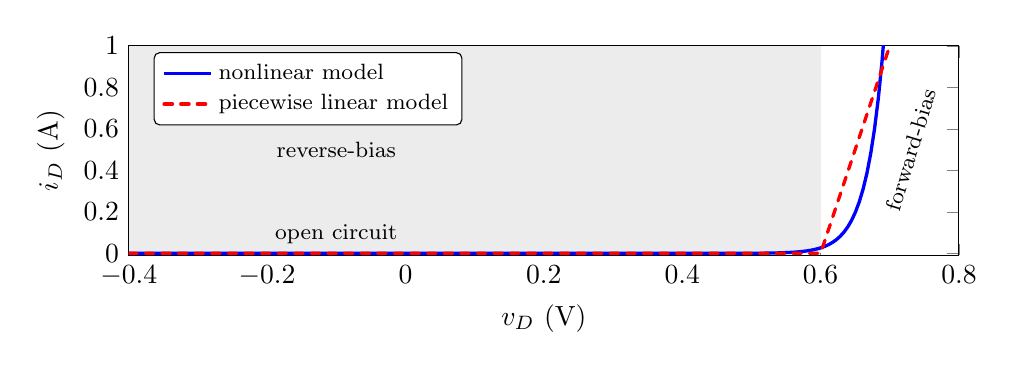
\begin{tikzpicture}[]
\usepgfplotslibrary{fillbetween}
\newcommand{\Is}{1e-12}
\newcommand{\VTH}{0.025}
\begin{axis}[
	width=1\linewidth,
	height=.35\linewidth,
	xmin=-.4,xmax=.8,
	ymin=-.01,ymax=1,
	xlabel=$v_D$ (V),
	ylabel=$i_D$ (A),
	legend entries={nonlinear model,piecewise linear model},
	legend style={
		legend pos=north west,
		cells={anchor=west},
		font=\footnotesize,
		rounded corners=2pt,
	}
]
\path[name path=yaxis](axis cs:-.4,0)-- (axis cs:-.4,1);
\path[name path=yaxis2](axis cs:.6,0)-- (axis cs:.6,1);
\addplot [
name path=plot,
blue,
very thick,
domain=-.4:.7,
samples=201,
]
{\Is*(exp(x/\VTH) - 1)};
%
\addplot  [
red,
dashed,
line cap=round,
very thick,
line join=bevel,
] coordinates
{(-.4,0) (.6,0) (1.6,10)};
%
\addplot[gray!15] fill between[
  of=yaxis and yaxis2,
];
%
\node at (axis cs:-.1,0) [anchor=south,font=\footnotesize] {open circuit};
\node at (axis cs:-.1,.5) [anchor=center,font=\footnotesize] {reverse-bias};
\node at (axis cs:.73,.5) [anchor=center,rotate=73,font=\footnotesize] {forward-bias};
\end{axis}
\end{tikzpicture}
\caption{the voltage-current relationship in the nonlinear and piecewise linear models. In the figure, $R_d = 0.1\ \Omega$.}
\label{fig:diode_iv}
\end{figure}

\subsection{A piecewise linear model}
\tags{}

\setlength\intextsep{0pt}
\begin{wrapfigure}{r}{0.42\textwidth}
  \centering
  \begin{circuitikz}[]
    \draw
      (0,0) to[full diode,box,i=$i_D$,v=$v_D$] (2,0);
  \end{circuitikz}
  \caption{\label{fig:ideal_diode} circuit symbol for an ideal diode. Note that this is a nonstandard use of this symbol.}%
\end{wrapfigure}

An \keyword{ideal diode} is one that is a perfect insulator (open circuit, $i_D = 0$) for $v_D < 0$ conductor for $v_D > 0$.
We use the symbol shown in \cref{fig:ideal_diode} for the ideal diode.
At times, the ideal diode is sufficient to model a diode; often, however, we prefer a more accurate model that is piecewise linear.
\tags{}

\setlength\intextsep{0pt}
\begin{wrapfigure}{r}{0.42\textwidth}
  \centering
	\begin{circuitikz}[]
    \draw
      (0,0) to[full diode] ++(1.5,0)
      to[battery1,v=$ $,l=$0.6$ V] ++(1.5,0)
      to[resistor,R=$R_d$] ++(1.5,0);
	\end{circuitikz}
  \caption{\label{fig:piecewise_linear_diode} piecewise linear model.}%
\end{wrapfigure}

The \keyword{piecewise linear model} is shown in \autoref{fig:piecewise_linear_diode}.
It includes an ideal diode in series with a fixed voltage drop of $0.6$ V and a resistor with resistance $R_d$.
This approximates the nonlinear model with two linear approximations.
\tags{R, D}

\maybeeqn{piecewise linear diode model}{}{
	\begin{align*}
		i_D = 
		\begin{cases} 
      0 & \text{for } v_D \leq 0.6\ \text{V} \\
      \dfrac{v_D-0.6\ \text{V}}{R_d} & \text{for } v_D > 0.6\ \text{V}
	  \end{cases}
	\end{align*}
  \label{eq:diode_piecewise_linear}
}

See \autoref{fig:diode_iv} for a plot of this function and a comparison to the nonlinear model.
\tags{}

The slope in forward-bias is $1/R_d$.
This model's effectiveness is highly dependant on $R_d$, so an \keyword{operating point} must be chosen and $R_d$ chosen to match most closely with the nonlinear model near that operating point.
\tags{R, D}

\subsection{Method of assumed states}
\tags{}

The \keyword{method of assumed states} is a method for using linear circuit analysis to analyze circuits with nonlinear components.
The method is summarized in the following steps.
\tags{}
\begin{enumerate}
  \item Begin at the initial time $t=0$.
  \item Replace each diode in the circuit diagram with the piecewise linear diode model.
  \item Proceed with the circuit analysis of \cref{ch:circuitanalysis}, ignoring the elemental equations for the ideal diodes $D_i$. Your system of equations will have unknown ideal diode current $i_{D_i}$ and voltage $v_{D_i}$. Simplify it to the extent possible.
  \item Guess the current state of each ideal diode: \texttt{ON} or \texttt{OFF}. For each ideal diode $D_i$ guessed to be \texttt{ON},
  \begin{align}
    \text{set}\ v_{D_i} = 0 \quad 
    \text{and assume that} \quad
    i_{D_i} > 0.
  \end{align} 
  For each ideal diode assumed to be \texttt{OFF},
  \begin{align}
    \text{set}\ i_{D_i} = 0 \quad 
    \text{and assume that} \quad
    v_{D_i} < 0.
  \end{align} 
	For $n$ diodes in the circuit, there are $2^n$ possibilities at each moment in time. Guess just one to start.
	\item If \emph{even one diode} violates its assumption from above, dismiss the results and return to step 4 and choose a different combination of assumed states (consider flipping the assumptions on those diodes that violated the old assumptions).
  \item If \emph{not even one diode} violates its assumptions, \emph{this is the correct solution for this moment in time}.
  \item This solution is valid for as long as its assumptions are valid. Once they fail, go back to step 4.
\end{enumerate}

Since impedance methods are valid only for \emph{linear} circuits, steady-state analyses should proceed with the same process outlined above.
With a periodic input, a periodic (steady) solution may emerge.
\tags{}

\examplemaybe{%
	half wave rectifier
}{%
	\begin{minipage}[c]{.65\linewidth}
    Given the circuit shown with voltage source $V_s(t) = 3 \cos 2\pi t$, what is the output $v_R$? Explain why this might be called a ``half-wave rectifier.''
    Let $R = 10$ $\Omega$.
  \end{minipage}
  \hfill%
  \begin{minipage}[c]{.3\linewidth}
    \begin{circuitikz}[]
			\draw
				(0,0) to[voltage source, v=$V_s$] (0,2)
				to[diode, i=$i_{D}$] (2,2)
				to[R=$R$, i=$i_{R}$] (2,0)
				-- (0,0);
		\end{circuitikz}
  \end{minipage}
}{%
	\begin{minipage}[c]{.4\linewidth}
    Let's use the piecewise linear model, which can be drawn as shown. We use the method of assumed states. First, subcircuits.
  \end{minipage}
  \hfill%
  \begin{minipage}[c]{.5\linewidth}
    \begin{circuitikz}[]
			\draw
				(0,0) to[voltage source, v=$V_s$] (0,2)
				to[full diode, i=$i_{D}$] (1.5,2);
			\draw
				(4.5,2)	to[resistor,R=$R_d$] (3,2) 
				to[battery1,v=$0.6$ V] (1.5,2);
			\draw
				(4.5,2) to[R=$R$, i=$i_{R}$] (4.5,0)
				-- (0,0);
		\end{circuitikz}
  \end{minipage}
	\begin{minipage}[c]{.4\linewidth}
    At right, we have the subcircuit with the \emph{on} state of the ideal diode.
  \end{minipage}
  \hfill%
  \begin{minipage}[c]{.5\linewidth}
    \begin{circuitikz}[]
			\draw
				(0,0) to[voltage source, v=$V_s$] (0,2)
				to[short] (1.5,2);
			\draw
				(4.5,2)	to[resistor,R=$R_d$] (3,2) 
				to[battery1,v=$0.6$ V] (1.5,2);
			\draw
				(4.5,2) to[R=$R$, i=$i_{R}$] (4.5,0)
				-- (0,0);
		\end{circuitikz}
  \end{minipage}
	\begin{minipage}[c]{.4\linewidth}
    At right, we have the subcircuit with the \emph{off} state of the ideal diode.
  \end{minipage}
  \hfill%
  \begin{minipage}[c]{.5\linewidth}
    \begin{circuitikz}[]
			\draw
				(0,0) to[voltage source, v=$V_s$] (0,2)
				to[open,o-o] (1.5,2);
			\draw
				(4.5,2)	to[resistor,R=$R_d$] (3,2) 
				to[battery1,v=$0.6$ V] (1.5,2);
			\draw
				(4.5,2) to[R=$R$, i=$i_{R}$] (4.5,0)
				-- (0,0);
		\end{circuitikz}
  \end{minipage}

  Now, to analyze each circuit.
  The on circuit, if we consider the dc voltage source to be an offset of the ac source, it is a voltage divider:
  \begin{align*}
  	v_R &= \frac{R}{R+R_d} (V_s-0.6).
  \end{align*}
  The value of $R_d$ is tbd.
  Let's use a thought experiment to decide what range of current for which we might need $R_d$ to be valid.
  We know that
  \begin{align*}
  	i_D 
  	&= i_R \\
  	&= v_R/R. 
  \end{align*}
  If $R_d = 0$, the maximum value of $v_R$ is $3-0.6 = 2.4$ V.
  Therefore,
  \begin{align*}
  	i_{D\text{max}} &= 2.4/10 \\
  	&= 0.24\text{ A}.
  \end{align*}
  From \autoref{fig:diode_iv}, we can choose a reasonable value of $R_d = 0.2\ \Omega$.
  Now that we have $R_d$, so we now have our on solution:
  \begin{align*}
  	v_R &= \frac{10}{10+0.2} (3 \cos 2\pi t - 0.6) \\
  	&\approx 2.94 \cos 2\pi t - 0.588.
  \end{align*}
  The off solution for $v_R$ is $v_R = i_R R = (0) R = 0$ V.
  To determine which solution is valid, we need to determine when the on solution predicts $i_D < 0$.
  Since $i_D = i_R = v_R/R$,
  \begin{align*}
  	i_D &= 0.294 \cos 2\pi t - 0.0588
  \end{align*}
  which is positive for an interval each period.
  The endpoints of the interval correspond to
  \begin{align*}
  	0 &= 0.294 \cos 2\pi t - 0.0588 \\
  	t &= \pm\frac{1}{2\pi}\arccos{0.2} \pm T \\
  	&= \pm 0.218\ \pm T \text{ sec}
  \end{align*}
  where $T \in \mathbb{N}_0$ is the period.
  The function is positive between these points in each period.
  Therefore, for all positive intervals, the on solution is correct, and for all negative intervals, the off solution is correct.

  Consider \autoref{fig:half_wave_rectifier}. The voltage output is always positive, but the effects of the non-ideality of the diode are apparent with the voltage offset and the (slight) scaling.

  This circuit is called the half-wave rectifier because it gives approximately the upper-half of the wave at its output.
  This introduces a dc offset.
  With some filtering, this can be used as an ac-to-dc rectifier.
  Note that typically a \emph{full-wave bridge rectifier} is used for this application.
}{%
ex:half_wave_rectifier%
}

\begin{figure}[b]
\centering
\begin{tikzpicture}[]
\pgfplotsset{set layers}
\begin{axis}[
	scale only axis,
	axis y line*=left,
	ylabel style = {align=center},
	ylabel={input $V_s$ (V) \ref{pgfplots:Vs} \\ output $v_R$ (V) \ref{pgfplots:vR}},
	width=.7\linewidth,
	height=.5\linewidth,
	xmin=-1,xmax=1,
	ymin=-3.1,ymax=3.1,
	xlabel=time (s),
]

\addplot [
blue,
very thick,
domain=-1:1,
samples=201,
]
{3*cos(2*pi*deg(x))};
\label{pgfplots:Vs}
\addplot [
red,
very thick,
domain=-.218:.218,
samples=201,
]
{2.94*cos(2*pi*deg(x))-0.588};
\label{pgfplots:vR}
\addplot [
red,
very thick,
domain=-1.218:-.782,
samples=201,
]
{2.94*cos(2*pi*deg(x))-0.588};
\addplot [
red,
very thick,
domain=.782:1.218,
samples=201,
]
{2.94*cos(2*pi*deg(x))-0.588};
\addplot [
red,
very thick,
domain=.218:.782,
samples=201,
]
{0};
\addplot [
red,
very thick,
domain=-.218:-.782,
samples=201,
]
{0};

\end{axis}
%
\begin{axis}[
	scale only axis,
	axis y line*=right,
	ylabel style = {align=center},
	ylabel={\emph{on} diode current $i_D$ (A) \ref{pgfplots:iD}},
	width=.7\linewidth,
	height=.5\linewidth,
	xmin=-1,xmax=1,
	ymin=-.5,ymax=.5,
]

\addplot [
mygreen,
very thick,
domain=-1:1,
samples=201,
]
{0.294*cos(2*pi*deg(x))-0.0588};
\label{pgfplots:iD}

\end{axis}
\end{tikzpicture}
\caption{the input and output voltage of the half-wave rectifier circuit of \autoref{ex:half_wave_rectifier}. Note that the ``on'' diode subcircuit is valid for $i_D > 0$ and the ``off'' diode circuit is valid for $i_D < 0$.}
\label{fig:half_wave_rectifier}
\end{figure}

\subsection{An algorithm for determining $R_d$}
\tags{}

The piecewise linear approximation of the exponential diode current will never be great, but we can at least try to choose $R_d$ in a somewhat optimal way, recognizing that when highly accurate results are required, there's no substitute for the nonlinear model.
\tags{R, D}

Consider the algorithm of \cref{fig:diode_resistance_algorithm}.
Initially set to zero the diode resistances $R_{d_i}$ of each resistor.
Solve for each diode current $i_{D_i}(t)$, then use this to find $v_{D_i}(t)$ from the
\emph{nonlinear} model of \cref{eq:diode_nonlinear}:
\tags{R, D}

\begin{align}
  \label{eq:diode_nonlinear_for_v}
  v_{D_i}(t) = V_\text{TH}
    \ln(
      i_{D_i}(t)/I_s + 1
    ).
\end{align}

Now take the means of these signals (assuming steady state oscillation) over a period $T$, excluding the time $T_0$ during which the diode voltage was in reverse-bias:\footnote{Note that if $T_0$ is ignored, our estimate of $R_d$ will include the effects of time during which no current is flowing and the diode is in reverse-bias, during which time $R_d$ is not applicable.}
\tags{R, D}

\begin{subequations}
\begin{align}
  \overline{i}_{D_i} = \frac{1}{T-T_0}
    \int_{t_0}^{t_0+T} i_{D_i}(\tau) d\tau \\
  \overline{v}_{D_i} = \frac{1}{T-T_0}
    \int_{t_0}^{t_0+T} v_{D_i}(\tau) d\tau. 
\end{align}
\end{subequations}

\begin{figure}
\centering
\usetikzlibrary{shapes,arrows}
% Define block styles
\tikzstyle{decision} = [
  diamond, 
  draw, 
  thick,
  % fill=blue!20, 
  text width=4.5em, 
  text badly centered, 
  node distance=3cm, 
  inner sep=.25em, 
]
\tikzstyle{block} = [
  rectangle, 
  draw, 
  thick,
  % fill=blue!20, 
  % text width=12em, 
  text centered, 
  rounded corners, 
  inner sep=.5em, 
  % minimum height=2em
]
\tikzstyle{line} = [
  draw, 
  thick,
  % -latex',
  ->,
]
\tikzstyle{cloud} = [draw, ellipse,fill=red!20, node distance=3cm, inner sep=1em]
{\sffamily
\begin{tikzpicture}[node distance = 1.25cm, auto]
  % place nodes
  \node[block] (n1) {analyze circuit with $R_{d_i}$ undetermined};
  \node[block,below of=n1] (n2) {let $R_{d_i} = 0$};
  \node[block,below of=n2] (n3) {solve for $i_{D_i}(t)$};
  \node[block,below of=n3] (n4) {use nonlinear model to find $v_{D_i}(t)$};
  \node[block,below of=n4] (n41) {find means $\overline{i}_{D_i}$, $\overline{v}_{D_i}$};
  \node[block,below of=n41] (n5) {use linear model to find $R_{d_i}$};
  \node[decision,right of=n5, node distance=12em] (d1) {$R_{d_i}$\\ converged?};
  \node [block, right of=d1, node distance=7em] (stop) {stop};
  % draw edges
  \path[line] (n1) -- (n2);
  \path[line] (n2) -- (n3);
  \path[line] (n3) -- (n4);
  \path[line] (n4) -- (n41);
  \path[line] (n41) -- (n5);
  \path[line] (n5.east) -- (d1.west);
  \path[line] (d1.east) -- (stop.west);
  \path[line] (d1.north) |- (n3);
\end{tikzpicture}
}
\caption{an algorithm for determining $R_{d_i}$.}
\label{fig:diode_resistance_algorithm}
\end{figure}

Now us the piecewise linear model of \cref{eq:diode_piecewise_linear} to estimate $R_{d_i}$:
\tags{R, D}

\begin{align}
  R_{d_i} = \frac{\overline{v}_{D_i}-0.6 V}{\overline{i}_{D_i}}.
\end{align}

We can use this estimate of $R_{d_i}$ to re-analyze the circuit and repeat the same process of deriving a new estimate of $R_{d_i}$.
This process should converge on an estimate of $R_{d_i}$ that is in some sense optimal.
\tags{R, D}

Note that if, during this iterative process, one finds $\overline{v}_{D_i} < 0.6$ V, a \emph{negative} $R_d$ will result.
At this point, a couple different reasonable approaches can be taken:
\tags{R, D}

\begin{enumerate}
  \item just use $R_{d_i} = 0$ or
  \item use some reasonably central value of $\overline{v}_{D_i} > 0.6$ V.
\end{enumerate}

The second case is preferred if $v_{D_i}(t)$ spends much time above $0.6$ V.
But usually, if it spends much time, the mean $\overline{v}_{D_i}$ should be great enough to avoid this situation.
Circuits that tend to express this behavior are those with high impedance and correspondingly low currents.
\tags{V, I, S}

\section{MOSFETs}
\tags{}

A metal–oxide–semiconductor field-effect transistor (MOSFET) is a \emph{two-port}, \emph{nonlinear} circuit element that lies at the heart of digital electronics, with sometimes millions integrated into a single microprocessor.
They are the dominant type of \keyword{transistor}, a class of elements that includes the \keyword{bipolar junction transistor (BJT)}.
\tags{}

MOSFETs are not just common in integrated circuits made of silicon, they are also available as discrete elements, which is the form most often encountered by the mechatronicist.
\tags{}

There are two primary types of MOSFET: the \keyword[n-channel MOSFET]{n-channel} and the \keyword[p-channel MOSFET]{p-channel}, determined by the type of semiconductor doping (negative or positive) used in the manufacturing process.
These types are ``opposites,'' so we choose to focus on n-channel, here.
\tags{}

\setlength\intextsep{0pt}
\usetikzlibrary{arrows,shapes,calc,positioning}
\begin{wrapfigure}{r}{0.35\textwidth}
  \centering
	\begin{circuitikz}[]
		\draw (0,0) node[nmos](T){};
		\draw (T.gate) --++(-.05,0) node[left] {$G$};
		\draw (T.drain) --++(0,.05) node[below right] {$D$};
		\draw (T.source) to[short,i_=$i_{DS}$] ++(0,-.05) node[above right] {$S$};
   	% \draw(T.gate) to[open,v={$v_{GS}$}] ++(0,-1);
   	% \draw(T.drain) to[open,v={$v_{DS}$}] (T.source);
	\end{circuitikz}
  \caption{\label{fig:nmosfet} circuit symbol for a n-channel MOSFET.}%
\end{wrapfigure}

\autoref{fig:nmosfet} displays the circuit diagram symbol for the MOSFET.
There are three\footnote{Note that if we consider the gate-side to be the input with $i_{GS}=0$ and $v_{GS}$ and the drain-source-side to be the output with $i_{DS}$ and $v_{DS}$, the MOSFET can be seen to be two-port.} terminals: the \keyword{gate $G$}, \keyword{drain $D$}, and \keyword{source $S$}.
The current flowing from one terminal to another is labeled with consecutive subscripts; for instance, the current flowing from drain to source is $i_{DS}$.
Similarly, the voltage drop across two terminals is labeled with concurrent subscripts; for instance, the voltage drop from gate to source is $v_{GS}$.
\tags{V, I, S}

The input-output characteristics of the MOSFET are quite complex, but we may, in the first approximation, consider it to be like a \emph{switch}.
In this model, called the \keyword[switch S-model]{S-model}, if the gate voltage $v_{GS}$ is less than the \keyword{threshold voltage} $V_T$ (typically around $0.7$ V), the $D$ and $S$ terminals are disconnected (open) from each other (OFF mode).
But when $v_{GS} > V_T$, $D$ and $S$ are connected via a short and current $i_{DS}$ can flow (ON mode).
\tags{V, I, S}

The input-output characteristics of a MOSFET are actually much more complex than the S-model captures.
The S-model can build intuition and suffice for digital logic circuit analysis.
However, we are here mostly concerned with analog circuit models.
Specifically, we mechatronicists use MOSFETs to drive power-hungry loads (e.g.\ motors) with high-power sources controlled by low-power microcontrollers.
We now turn to a general model, after which we consider a method of analyzing MOSFET circuits.
\tags{}

\subsection{The switch unified (SU) model}
\tags{}

The \keyword{switch unified (SU) model} is reasonably accurate at describing actual MOSFET input-output characteristics.
However, it is quite \emph{nonlinear}, and therefore can give us headaches during analysis.
As usual, we are concerned with the element's voltage-current relationships.
\tags{V, I, S}

\begin{Definition}{switch unified model}{sumodel}
	Let $K$ be a constant parameter of the MOSFET with units $\text{A}/\text{V}^2$.
	$K$ can be found from parameters of a given MOSFET.
	The current into the gate is zero: $i_{G} = 0$.
	The current from drain to source is controlled by the two voltage variables $v_{GS}$ and $v_{DS}$, as shown.
	\begin{align*}
		i_{DS} =
		\begin{cases}
			0 & 
			\text{for } v_{GS} < V_T \\
			K
			\left(
				(v_{GS}-V_T) v_{DS} - v_{DS}^2/2
			\right) & 
			\text{for } v_{GS} \ge V_T \text{ and } v_{DS} < v_{GS} - V_T \\
			\dfrac{K}{2}(v_{GS}-V_T)^2 & 
			\text{for } v_{GS} \ge V_T \text{ and } v_{DS} \ge v_{GS} - V_T
		\end{cases}
	\end{align*}
\end{Definition}

So, as in the S-model, the gate voltage $v_{GS}$ must exceed the threshold voltage $V_T$ for current to flow.
The interval below the threshold is called the \keyword{cutoff region} (OFF).
Note, however, that current doesn't just flow freely, as it would with the short of the S-model.
In fact, two distinct ON ($v_{GS}>V_T$) intervals emerge.
In both, the current $i_{DS}$ depends on $v_{GS}$.
In the \keyword{triode region}, $v_{DS}<v_{GS} - V_T$, $i_{DS}$ also depends on $v_{DS}$.
However, in the \keyword{saturation region}, $v_{DS}>v_{GS} - V_T$, $i_{DS}$ is independent of $v_{DS}$ and can be controlled by $v_{GS}$, alone.
\tags{V, I, S}

Note that in saturation, the MOSFET behaves like a current source controlled by $v_{GS}$.
A source controlled by a variable in the circuit is called a \keyword{dependent source}.
This behavior as a dependent current source (that can also be turned off) is the most valuable for us.
\tags{V, S}

The \keyword{switch current source (SCS) model} is actually just a recognition of this behavior and an elimination of the triode region from consideration.
This is a reasonable assumption if we can guarantee operation in cutoff or saturation only.
\tags{}

Given the piecewise MOSFET models, we can again use the \keyword{method of assumed states} for MOSFET circuit analysis.
Note however that only the S-model is piecewise linear and that the SU- and SCS-models are piecewise nonlinear.
We can handle some relatively simple nonlinear cases analytically, but require either linearization or numerical assistance for more complex circuit analyses.
\tags{}
%TODO ... 2018 I may have done this ... 2017 method of solving from Agarwal (assuming saturation) ... should be like the diode method, I think?

\usetikzlibrary{calc}
\examplemaybe{%
	transformers and impedance
}{%
	\begin{minipage}[c]{.45\linewidth}
    Given the circuit shown, solve for the voltage across the load $R_L$ for varying $V_g$ given the following conditions: saturation of the MOSFET, $R_L = 1$ k$\Omega$, $K = 0.5\ \text{mA}/\text{V}^2$, $V_T = 0.7$ V, $V_s = 10$ V.
  \end{minipage}
  \hfill%
  \begin{minipage}[c]{.5\linewidth}
		\begin{circuitikz}[]
			\draw (0,0) node[nmos](T){};
			\coordinate (Vs) at ($(T.drain)+(0,1.5)$);
			\draw (Vs) to[R,l_=$R_L$,i_=$i_{R_L}$] (T.drain);
			\draw (T.source) --++(1.5,0)
				coordinate (foo)
				to[voltage source,v,l_=$V_s$] (foo |- Vs)
				-- (Vs);
			\draw (T.source) --++(-2,0)
				to[voltage source,v,l=$V_g$] ++(0,1.5)
				-- ++(.75,0)
				coordinate (bar)
				-- (bar |- T.gate)
				-- (T.gate);
		\end{circuitikz}
  \end{minipage}
}{%
	During saturation,
	\begin{align*}
		i_{DS} = \dfrac{K}{2}(v_{GS}-V_T)^2.
	\end{align*}
	We know that $v_{GS} = V_g$ and the other parameters are given.
	The voltage across the resistor is, from Ohm's law,
	\begin{align*}
		v_{R_L} = i_{R_L} R_L.
	\end{align*}
	From KCL,
	\begin{align*}
		v_{R_L} &= i_{DS} R_L \\
		&= \dfrac{K R_L}{2}(V_g-V_T)^2.
	\end{align*}
	This is our load voltage, but we must determine the range of $V_g$ for which saturation is satisfied.
	We must first find $v_{DS}$. From KVL,
	\begin{align*}
		v_{DS} &= V_s - v_{R_L} \\
		&= V_s - \dfrac{K R_L}{2}(V_g-V_T)^2.
	\end{align*}
	The condition for saturation (in addition to $V_g>V_T$) is
	\begin{align*}
		v_{DS} &\ge v_{GS} - V_T \quad\Rightarrow \\
		V_s - \dfrac{K R_L}{2}(V_g-V_T)^2 &\ge V_g - V_T \quad\Rightarrow \\
		V_T - \frac{1+\sqrt{2 K R_L V_s}}{K R_L} &\le
		V_g \le
		V_T + \frac{-1+\sqrt{2 K R_L V_s}}{K R_L}.
	\end{align*}
	Since $V_g>V_T$, we can simplify the condition for saturation to
	\begin{align*}
		V_T < V_g \le
		V_T + \frac{-1+\sqrt{2 K R_L V_s}}{K R_L}.
	\end{align*}
	Computing the upper bound, we obtain $5.33$ V.
	See \autoref{fig:mosfet_example} for the plot.
	Note that the similar input and load voltage might suggest we didn't need to MOSFET.
	However, the input voltage has virtually zero load, whereas the source voltage does.
	Essentially, the current draw (and therefore power) is different!
	We're controlling a constant, more powerful source with a weaker, (ideally) variable source.
}{ex:mosfet}

\begin{figure}[bt]
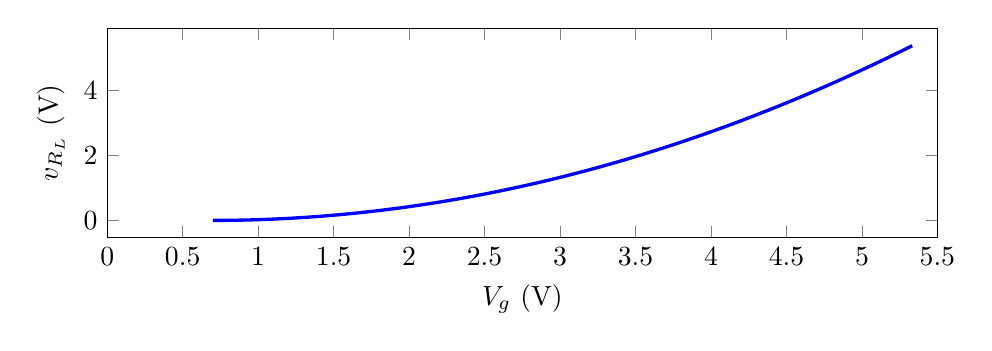
\begin{tikzpicture}[]
\newcommand{\Know}{5e-4}
\newcommand{\RL}{1e3}
\newcommand{\VT}{0.7}
\begin{axis}[
	width=1\linewidth,
	height=.35\linewidth,
	xmin=0,xmax=5.5,
	% ymin=-.01,ymax=1,
	xlabel=$V_g$ (V),
	ylabel=$v_{R_L}$ (V),
	% legend entries={nonlinear model,piecewise linear model},
	% legend style={
	% 	legend pos=north west,
	% 	cells={anchor=west},
	% 	font=\footnotesize,
	% 	rounded corners=2pt,
	% }
]
\addplot [
blue,
very thick,
domain=.7:5.333,
samples=201,
]
{\Know*\RL/2*(x-\VT)^2};
\end{axis}
\end{tikzpicture}
\caption{the load voltage as a function of gate voltage for \autoref{ex:mosfet}.}
\label{fig:mosfet_example}
\end{figure}

\section{Operational amplifiers}
\tags{}

The \keyword{operational amplifier} (opamp) is the queen of analog electronic components.
The opamp is a \emph{four-port nonlinear} voltage-controlled voltage source, but it's so much more.
Here are a few applications from the opamp highlight reel: summing two signals, subtracting two signals, amplifying a signal, integrating a signal, differentiating a signal, filtering a signal, isolating two subcircuits, generating periodic functions (e.g.\ sinusoids and square waves), and analog feedback control.
Although they are nonlinear, in most applications a linear approximation is sufficiently accurate.
\tags{}


\setlength\intextsep{0pt}
\usetikzlibrary{arrows,shapes,calc,positioning}
\begin{wrapfigure}{r}{0.35\textwidth}
  \centering
	\begin{circuitikz}[]
		\draw (0,0) node[op amp](opamp){}
   	(opamp.+) node[left] {$v_+$}
		(opamp.-) node[left] {$v_-$}
		(opamp.out) node[right] {$v_o$};
	\end{circuitikz}
  \caption{\label{fig:opamp} circuit symbol for an opamp.}%
\end{wrapfigure}
\autoref{fig:opamp} shows the circuit symbol for the opamp.
Three terminals are displayed:
\begin{description}
	\item[inverting input ($-$)] The \keyword[inverting input ($-$)]{inverting input} is labeled with the ``$-$'' symbol.
	\item[non-inverting input ($+$)] The \keyword[non-inverting input ($+$)]{non-inverting input} is labeled with the ``$+$'' symbol.
	\item[output] The \keyword{output} extends from the tip of the symbol, opposite the inputs.
\end{description}

These comprise an input and an output port.
However, there are two power supply ports that are typically suppressed in the circuit diagram.
These two power supply ports are from a \keyword[differential power supply]{differential supply}, which has a positive terminal (e.g.\ $+12$ V), symmetrically negative terminal (e.g.\ $-12$ V), and a common ground.
The supply provides the opamp with external power, making it an \keyword[active element]{active} element.
\tags{}

When an opamp is operating in its linear mode, it outputs a voltage $v_o$ that is $A$ times the difference between its inputs $v_+$ and $v_-$.
The \keyword{open-loop gain $A$} is different for every opamp, but is usually greater than $10^5$.
Let's formalize this model.
\tags{V, S}

\begin{Definition}{opamp model}{opamp}
	An opamp's input terminals $+$ and $-$ draw zero current (i.e.\ have infinite input impedance).
	Let $A$ be a positive real number.
	The output voltage $v_o$ is given by
	\begin{align*}
		v_o = A (v_+ - v_-).
	\end{align*}
	The output terminal has zero impedance.
\end{Definition}

Note that this model is equivalent to a \keyword{dependent voltage source} controlled by the input voltage difference.
In fact, it is also \emph{linearly} dependent, so linear circuit analysis techniques can be applied.\footnote{Note that, while the transistor can be considered a nonlinear dependent current source, the opamp can be considered a linear dependent voltage source. However, we can easily adapt an opamp circuit to behave as a linear dependent current source, so typically the opamp is still preferred.}
\tags{S, V}

The model is fairly accurate as long as $|v_o|$ is less than the maximum power source voltage.
Due to the high open-loop gain, the difference in input gain is highly restrictive for linear operation.
This turns out not to be difficult to achieve, but does lead to a convenient approximation during analysis that applies most of the time:
\tags{S, V}

\begin{align}
	\label{eq:v_plus_minus}
	v_+ \approx v_-
\end{align}

because other voltages in the circuit are typically much larger than the input voltage difference.
We cannot, however, make this assumption unless (1) the opamp is operating in linear mode and (2) the opamp is part of a circuit that connects its output---via a wire or circuit elements---back to its inverting input ($-$).
\tags{V, S}

This second condition is called \keyword{negative feedback} and is used in most opamp circuits for several reasons, the most important of which is that \autoref{eq:v_plus_minus} holds due to the virtual guarantee of linear operation in this case.
\tags{}

\subsection{Negative feedback}
\tags{}

We can think of negative feedback as continuously adjusting the output such that \autoref{eq:v_plus_minus} is approximately true.\footnote{Negative feedback is considered in detail in courses on control theory. The opamp was used extensively for feedback control until low-cost, high-performance digital microcontrollers became available. Opamp-based feedback control is now called \emph{analog feedback control}, which still has certain applications.}
Consider the feedback of $v_o$ to the inverting input (called \keyword{unity feedback}), as shown in \autoref{fig:opamp2}, such that the output equation can be transformed as follows:
\tags{}
\maybeeq{
	\begin{align*}
		v_o &= A (v_+ - v_-) \\
		&= A (v_i - v_o) \quad \Rightarrow \\
		v_o &= \frac{A}{1+A} v_i
	\end{align*}
}

Since $A \gg 1$, $v_o \approx v_i$.
In other words, \emph{for negative unity feedback, $v_o$ follows $v_i$}.
For this reason, this particular opamp circuit is called a \keyword{voltage follower}.
Let's consider negative feedback's effect on the difference in input voltage:
\tags{V, S}

\maybeeq{
	\begin{align*}
		v_+ - v_- &= v_+ - \frac{A}{1+A} v_+ \\
		&\approx 0.
	\end{align*}
}

This is equivalent to \autoref{eq:v_plus_minus}.
That is, \emph{for negative feedback, the input voltages are nearly equal:} $v_+ \approx v_-$.
This is control theory---this is how we make a system behave the way we want!
In this instance, the \keyword{loop gain}---the effective gain from $v_i$ to $v_o$---is one.
This same principle applies when elements such as resistors and capacitors are placed in the feedback path.
The resulting loop gain can be nonunity and respond dynamically to the signal.
\tags{V, S}

\subsection{Non-inverting opamp circuit}
\tags{}

\begin{figure}[t]
  \centering
  \subbottom[\label{fig:opamp2} negative unity feedback controlling the voltage across an element $Z$.]{%
  \begin{circuitikz}[]
    \draw (0,0) node[op amp,yscale=-1](opamp){}
    (opamp.out) node[above] {$v_o$}
    (opamp.out) -- ++(1,0)
    to[generic,label=$Z$] ++(0,-1.5)
    node[ground]{}
    (opamp.out) -- ++(0,-1.5)
    coordinate (foo) 
    -- (foo -| opamp.-)
    -- (opamp.-);
    \draw (-2,-1.5)
    node[ground](g){}
    to[voltage source,label=$v_i$] (g |- opamp.+)
    -- (opamp.+);
  \end{circuitikz}%
  }
  \quad
  \subbottom[\label{fig:opamp3} the non-inverting opamp circuit.]{%
	\begin{circuitikz}[]
		\draw (0,0) node[op amp,yscale=-1](opamp){}
		(opamp.out)	to[R,l_=$R_1$,i=$$] ++(0,-1.75)
		coordinate (mid) 
		to[R,l_=$R_2$,i=$$] ++(0,-1.75)
		coordinate (g2);
		\draw	(mid)	-- (mid -| opamp.-)
		-- (opamp.-);
		\draw (-2.5,-3.5)
		node[ground](g){}
		to[voltage source,label=$v_i$] (g |- opamp.+)
		-- (opamp.+);
		\draw (g) -- (g2);
		\draw (opamp.out) -- ++(.5,0)
		node[circ](bar){}
		to[open,v^=$v_o$] (bar |- g2)
		node[circ]{}
		-- (g2);
	\end{circuitikz}%
  }
  \caption{two opamp circuits.}
\end{figure}

The \keyword{non-inverting opamp circuit} is shown in \autoref{fig:opamp3}.
Let's analyze the circuit to find $v_o(v_i)$.
We begin with the KVL expression for $v_o$ in terms of $v_{R_1}$ and $v_{R_2}$:
\tags{V, R, S, D}

\maybeeq{
	\begin{align*}
		v_o &= v_{R_1} + v_{R_2}.
	\end{align*}
}
Let's use Ohm's law to write:
\maybeeq{
	\begin{align*}
		v_o &= i_{R_1} R_1 + i_{R_2} R_2.
	\end{align*}
}

The KCL equation for the node between $R_1$ and $R_2$ gives
\maybeeq{
	\begin{align*}
		i_{R_1} - i_{R_2} - \cancelto{0}{i_-} &= 0 \quad\Rightarrow \\
		i_{R_1} &= i_{R_2} \quad \Rightarrow \\
		v_o &= i_{R_2} (R_1 + R_2) \quad \Rightarrow \\
		i_{R_2} &= v_o/(R_1 + R_2).
	\end{align*}
}
We can write another equation for $v_o$ from the opamp:
\maybeeq{
	\begin{align*}
		v_o &= A (v_+ - v_-) \\
		&= A (v_i - v_{R_2}).
	\end{align*}
}
We have an expression for $i_{R_2}$ that can eliminate $v_{R_2}$ with a little Ohm's law action:
\tags{V, I, R, S, D}

\maybeeq{
	\begin{align*}
		v_o &= A (v_i - i_{R_2} R_2) \\
		&= A (v_i - v_o R_2/(R_1 + R_2)) \quad\Rightarrow \\
		v_o + v_o A R_2/(R_1+R_2) &= A v_i \\
		v_o &= \frac{A}{1+A R_2/(R_1+R_2)} v_i \\
		&= \frac{(R_1 + R_2)/R_2}{(R_1 + R_2)/(R_2 K)+1} v_i.
	\end{align*}
}
If $A\gg (R_1 + R_2)/R_2$, the denominator of this expression goes to $1$ and we have the loop gain approximately
\tags{R, D}

\maybeeq{
	\begin{align*}
		\frac{R_1 + R_2}{R_2}.
	\end{align*}%
}%

This gives the following input-output equation for the circuit.
\maybeeqn{non-inverting opamp circuit i/o equation}{eq:noninverting_io}{	
	\begin{align*}
		v_o \approx \frac{R_1 + R_2}{R_2} v_i
	\end{align*}
}%

It is highly significant that \autoref{eq:noninverting_io} doesn't depend on $A$, which can be quite variable.
Rather, it depends on the resistances $R_1$ and $R_2$, only---and these are very reliable.
As long as the condition
\tags{R, I, S, D}
\begin{align}
	A\gg\frac{R_1 + R_2}{R_2}
\end{align}
is satisfied, \autoref{eq:noninverting_io} is valid.

This independence of the input-output relationship on the open-loop gain $A$ is very common for opamp circuits.
We have essentially traded gain for better linearity and gain invariance.
It can be shown that this is equivalent to the assumption that $v_+ \approx v_-$.
Making this assumption earlier in the analysis can simplify the process.
Note that we do not use the assumption for the opamp equation $v_o = A (v_+ - v_-)$, for this would imply $v_o = 0$. 
Instead, in the previous analysis, we could immediately assume that $v_{R_2} = v_i$ and proceed in a similar fashion.
\tags{}

\begin{exercises}
\input{ch04_exercises}
\end{exercises}

\end{document}
